% LaTeX source for ``Algorithms for Computer Simulation of Molecular Systems''
% Copyright (c) 2023 รังสิมันต์ เกษแก้ว (Rangsiman Ketkaew).

% License: Creative Commons Attribution-NonCommercial-NoDerivatives 4.0 International (CC BY-NC-ND 4.0)
% https://creativecommons.org/licenses/by-nc-nd/4.0/

\chapter{กลศาสตร์ควอนตัมเชิงโมเลกุล}
\label{ch:mol_qm}

%----------------------------------------
\section{การจำลองเชิงตัวเลขและเทคนิคเชิงคอมพิวเตอร์}
%----------------------------------------

การจำลองเชิงตัวเลข (Numerical Modeling) คือวิธีที่การที่เราใช้ปัญหาทางคณิตศาสตร์และฟิสิกส์แบบต่าง ๆ เช่น นำมาใช้แก้สมการเชิง%
อนุพันธ์ที่ใช้ในการอธิบายปรากฏการณ์ต่าง ๆ ทางธรรมชาติซึ่งอาจจะมีความยากหรืออาจจะไม่มีทางแก้ได้ด้วยวิธีเชิงวิเคราะห์ (Analytical Method)
\idxboth{การจำลองเชิงตัวเลข}{Numerical Modeling}
\idxboth{วิธีเชิงวิเคราะห์}{Analytical Method}

สำหรับการจำลองด้วยเทคนิคเชิงคอมพิวเตอร์ (Computer Simulation) นั้นเป็นการศึกษาการตอบสนองเชิงพลวัต (Dynamic Response) 
ของระบบแบบจำลองต่อเงื่อนไขเริ่มต้น (Initial Conditions) ที่เราได้กำหนดไว้ โดยเงื่อนไขเริ่มต้นนี้สอดคล้องกับสภาวะจริงของระบบนั้น
\idxboth{เทคนิคเชิงคอมพิวเตอร์}{Computer Simulation}
\idxboth{เงื่อนไขเริ่มต้น}{Initial Conditions}

\begin{figure}[htbp]
    \centering
    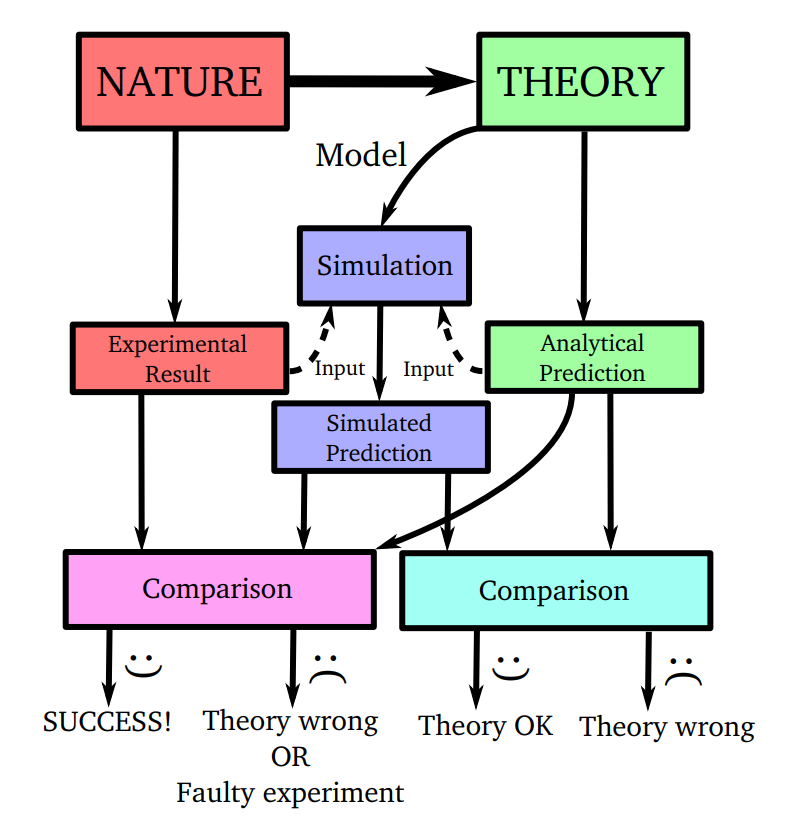
\includegraphics[width=0.8\linewidth]{fig/simulation-modeling-graph.png}
    \label{fig:sim_model_graph}
    \caption{แผนผังความเชื่อมโยงของระบบที่เราต้องศึกษา (Nature), ทฤษฎีหรือวิธีที่ใช้ในการศึกษา (Theory), แบบจำลองหรือโมเดล 
    (Model), ผลการทดลอง (Experimental Result), และผลการคำนวณหรือผลการทำนาย (Computational Results หรือ Prediction)}
\end{figure}

ภาพที่ \ref{fig:sim_model_graph} แสดงแผนผังเชื่อมโยงความแตกต่างระหว่าง Numerical Modeling กับ Computer Simulation 
นั้นก็คือใน Simulation นั้นระบบจำลองของเราจะถูกสร้างขึ้นมา เช่น เราสร้างระบบที่เป็นโมเลกุลน้ำหลาย ๆ โมเลกุลเกาะกลุ่มรวมกัน (Water 
Cluster) โดยเราหวังว่า Water Cluster ที่เราสร้างขึ้นมานี้จะสามารถเป็นตัวแทนของระบบของโมเลกุลน้ำจริง ๆ ได้ ซึ่งก็จะทำให้เราสามารถ%
ศึกษาคุณสมบัติต่าง ๆ ของโมเลกุลน้ำได้ตามต้องการ ส่วนการจำลองเชิงตัวหรือ Numerical Simulation นั้นจะเป็นการสร้างการทดลองเสมือนจริง 
(Virtual Experiments) ของระบบจำลองขึ้นมา อย่างไรก็ตามในบทความวิชาการทางด้านเคมีเชิงคำนวณหรือชีวเชิงคำนวณนั้นเรามักจะพบว่าคำว่า 
Modeling นั้นสามารถถูกแทนด้วยคำว่า Simulation ได้เช่นกัน

คำถามสำคัญที่หลายคนโดยเฉพาะอย่างนักวิทยาศาสตร์ที่ทำงานวิจัยเชิงการทดลองมักจะถามก็คือ \enquote{ทำไมการจำลองทางคอมพิวเตอร์ถึง%
มีความสำคัญ} คำตอบนั้นมีด้วยกันหลายข้อ ผู้เขียนขอสรุปเป็นประเด็นตามนี้ครับ

\begin{enumerate}
    \item การจำลองทางคอมพิวเตอร์นั้นเปรียบเสมือนเป็นสะพานเชื่อมโยงระหว่างทฤษฎีกับการทดลอง
    \item การทำการทดลองบางอย่างนั้นมีค่าใช้จ่ายที่สูงมากและมีความยากเพราะว่าตัวทฤษฎีนั้นซับซ้อนเกินไป ดังนั้นการจำลองทางคอมพิวเตอร์%
    นั้นจะเข้ามาช่วยในการจำลองการทดลองและทดสอบสมมติฐานเพื่อยืนยันทฤษฎีด้วย
    \item การจำลองทางคอมพิวเตอร์นั้นช่วยหาปัจจัยและเงื่อนไขที่เหมาะสมสำหรับการทดลองได้
    \item การจำลองทางคอมพิวเตอร์สามารถแสดงกระบวนการของระบบที่เราสนใจได้ ซึ่งอาจจะทำได้ยากในเชิงการทดลอง
    \item การจำลองทางคอมพิวเตอร์สามารถนำมาใช้ในการศึกษาปรากฏการณ์ที่การทดลองนั้นอาจจะให้ผลการทดลองที่ไม่ละเอียดพอ
\end{enumerate}

อย่างไรก็ตามผู้เขียนต้องขอสรุปเพิ่มเติมด้วยว่าการใช้แบบจำลองทางคอมพิวเตอร์เพียงอย่างเดียวนั้นจะเปล่าประโยชน์ถ้าหากว่าไม่มีผลการทดลองที่%
น่าเชื่อมายืนยันความถูกต้องของผลการคำนวณ ดังนั้นเคมีเชิงการทดลองกับเคมีเชิงคำนวณนั้นจึงเป็นศาสตร์ที่ต้องพึ่งพาอาศัยกัน
